\documentclass{beamer}

\usepackage{beamerthemesplit}
\usepackage{graphicx}
\usepackage{subfigure}
\usepackage{amsmath,amssymb}
\usepackage{multimedia}
\usepackage{times}

\usepackage[latin1]{inputenc}
\usepackage[T1]{fontenc}
\usepackage{listings}
\usepackage{courier}
\usepackage{color}

\newcommand{\re}{\text{Re}}
\newcommand{\im}{\text{Im}}
\newcommand{\de}{\mbox{d}}
\newcommand{\eref}[1]{(\ref{#1})}
\newcommand{\ii}{\text{i}}
\newcommand{\ee}{\text{e}}
\newcommand{\mathbi}[1]{\textbf{\em #1}}
\newcommand{\rem}[1]{}


% Layout specification

% \usetheme{AnnArbor}
% \usetheme{Antibes}
% \usetheme{Bergen}
% \usetheme{Berkeley}
% \usetheme{Berlin}
% \usetheme{Boadilla}
% \usetheme{boxes}
% \usetheme{CambridgeUS}
% \usetheme{Copenhagen}
% \usetheme{Darmstadt}
% \usetheme{default}
% \usetheme{Dresden}
% \usetheme{Frankfurt}
% \usetheme{Goettingen}
% \usetheme{Hannover}
% \usetheme{Ilmenau}
% \usetheme{JuanLesPins}
% \usetheme{Luebeck}
% \usetheme{Madrid}
% \usetheme{Malmoe}
% \usetheme{Marburg}
% \usetheme{Montpellier}
% \usetheme{PaloAlto}
% \usetheme{Pittsburgh}
% \usetheme{Rochester}
% \usetheme{Singapore}
% \usetheme{Szeged}
\usetheme{Warsaw}

% \usecolortheme{albatross}
% \usecolortheme{beaver}
% \usecolortheme{beetle}
% \usecolortheme{crane}
% \usecolortheme{default}
% \usecolortheme{dolphin}
% \usecolortheme{dove}
% \usecolortheme{fly}
% \usecolortheme{lily}
% \usecolortheme{orchid}
% \usecolortheme{rose}
% \usecolortheme{seagull}
% \usecolortheme{seahorse}
% \usecolortheme{sidebartab}
% \usecolortheme{structure}
% \usecolortheme{whale}
% \usecolortheme{wolverine}

% \usefonttheme{default}
% \usefonttheme{professionalfonts}
% \usefonttheme{serif}
% \usefonttheme{structurebold}
% \usefonttheme{structureitalicserif}
% \usefonttheme{structuresmallcapsserif}

% \useinnertheme{circles}
% \useinnertheme{default}
% \useinnertheme{inmargin}
% \useinnertheme{rectangles}
% \useinnertheme{rounded}

% \useoutertheme{default}
% \useoutertheme{infolines}
% \useoutertheme{miniframes}
% \useoutertheme{shadow}
% \useoutertheme{sidebar}
% \useoutertheme{smoothbars}
% \useoutertheme{smoothtree}
% \useoutertheme{split}
% \useoutertheme{tree}



% Meta

\title[odeint]{odeint}
\subtitle[odeint]{Solving ordinary differential equations in C++}
\author[Karsten Ahnert]{Karsten Ahnert$^{1,2}$ and Mario Mulansky$^2$}
\institute[Universit\"at Potsdam]{$^1$ Ambrosys GmbH, Potsdam\\ $^2$ Institut f\"ur Physik und Astronomie, Universit\"at Potsdam}
\date{\today}
%\logo{\pgfimage[width=2cm,height=2cm]{logo}}
\titlegraphic{\includegraphics[width=4cm]{ambrosys}\hspace{5ex}
\includegraphics[width=1.5cm,height=1.5cm]{logo}\hspace{7ex}
\includegraphics[height=1.5cm]{gsoc}}
\subject{Subject}
\keywords{Keyword1,Keyword2}



\definecolor{dark-gray}{gray}{0.15}
\definecolor{light-gray}{gray}{0.8}
\definecolor{lighter-gray}{gray}{0.9}

\definecolor{dark-green}{rgb}{0,0.4,0}
\definecolor{dark-red}{rgb}{0.2,0,0}



\lstset{
         basicstyle=\tiny\ttfamily, % Standardschrift
         %numbers=left,               % Ort der Zeilennummern
         numberstyle=\tiny,          % Stil der Zeilennummern
         %stepnumber=2,               % Abstand zwischen den Zeilennummern
         numbersep=5pt,              % Abstand der Nummern zum Text
         tabsize=2,                  % Groesse von Tabs
         extendedchars=true,         %
         breaklines=true,            % Zeilen werden Umgebrochen
         frame=single,         
         backgroundcolor=\color{lighter-gray},
         tabsize=4,
         keywordstyle=\color{dark-green},
         identifierstyle=,
         commentstyle=\color{dark-gray}\normalfont\rmfamily\itshape,
         stringstyle=\color{dark-red},
         showspaces=false,           % Leerzeichen anzeigen ?
         showtabs=false,             % Tabs anzeigen ?
         xleftmargin=17pt,
         xrightmargin=10pt,
         framexleftmargin=17pt,
         framexrightmargin=5pt,
         framexbottommargin=4pt,
         language=c++,
         showstringspaces=false      % Leerzeichen in Strings anzeigen ?        
 }
\lstloadlanguages{C++}




% What is shown

\beamertemplatenavigationsymbolsempty
\setbeamertemplate{footline}{}
% \setbeamertemplate{footline}{\insertframenumber}
\setbeamertemplate{headline}{}


\parindent0pt











\begin{document}



\frame{
  \titlepage


}

\frame{
  \frametitle{Outline}
  \tableofcontents
}


\section{Introduction}

\frame{
  \frametitle{The interface problem in C/C++}
  
    \begin{itemize}
      \item Many frameworks exist to do numerical computations.
      \item Data has to be stored in containers or collections.
      \item GSL: {\tt gsl\_vector}, {\tt gsl\_matrix}
      \item NR: pointers with Fortran-style indexing
      \item Blitz++, MTL4, boost::ublas
      \item QT: {\tt QVector}, wxWidgets: {\tt wxArray}, MFC: {\tt CArray}
    \end{itemize}

  %\vspace{2ex}

    {\bf \color{red} But:} All books on C++ recommend the use of the STL containers {\tt std::vector},
    {\tt std::list}, \dots

 \pause

  %\vspace{2ex}

  \begin{block}{Theoretical solution of the interface mess}
  GoF Design Pattern: Adaptor, also known as Wrapper

  % {\tiny Gamma, Holm, Johnson, Vlissides: {\it Design Patterns, Elements of Reuseable Object-Oriented Software},  1998.}
  \end{block}

  \pause

  \begin{exampleblock}{Alternative}
   Generic, container independent algorithms
  \end{exampleblock}

}

\frame{
  \frametitle{Example}
  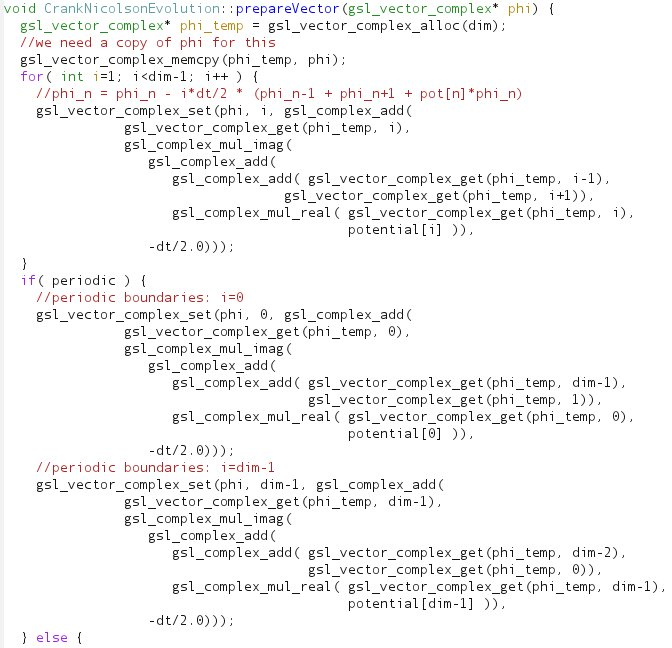
\includegraphics[draft=false,width=0.84\textwidth]{gsl_mess.jpg}
}

\frame{
  \frametitle{Portability of your algorithm}

  How to run your algorithm?
    \begin{itemize}
      \item Single machine, single CPU
      \item Single machine, multiple CPU's (OpenMP, threads, ...)
      \item Multiple machines (MPI)
      \item GPU (Cuda, Thrust, OpenCL)
    \end{itemize}

  \pause

  \vspace{2ex}

  Which data types are used by your algorithm?
   \begin{itemize}
    \item Build-in data types -- \texttt{double}, \texttt{complex<double>}
    \item Arbitrary precision types -- GMP, MPFR
    \item Vectorial data types \texttt{float2d}, \texttt{float3d}
   \end{itemize}

  \pause

  \vspace{2ex}

  \begin{block}{Theoretical solution}
    GoF Design Pattern: Strategy, also known as Policy
    
    {\tiny Gamma, Holm, Johnson, Vlissides: {\it Design Patterns, Elements of Reuseable Object-Oriented Software},  1998.}
  \end{block}
}

\frame{
  \frametitle{Numerical integration of ODEs}
  
    Find a numerical solution of an ODE an its initial value problem 
    \[ \dot{x} = f(x,t) \,\,\textrm{,} \quad \quad x(t=0) = x_0\]

   \vspace{2ex}

   Example: Explicit Euler
   \[ x(t + \Delta t ) = x(t) + \Delta t \,\, f(x(t),t) + \mathcal{O}(\Delta t^2)\]

   \vspace{2ex}

   General scheme of order $s$
    \[ x(t) \,\, \mapsto \,\, x(t+\Delta t) \quad \quad \text{, or}\]
    \[x(t + \Delta t) = \mathcal{F}_t x(t) + \mathcal{O}(\Delta t^{s+1})\]

}




\frame{
%  \frametitle{odeint - Solving ODEs in C++}

\centerline{\Large \bf \color{red}odeint}

\vspace{2ex}

\centerline{Solving ordinary differential equations in C++}

\vspace{2ex}

Open source
\begin{itemize}
\item Boost license -- do whatever you want do to with it 
\end{itemize}

\pause

\vspace{2ex}

Download
\begin{itemize}
\item \texttt{\textbf{www.odeint.com}}
% \item \texttt{https://github.com/headmyshoulder/odeint-v2}
\end{itemize}

\pause

\vspace{2ex}

Modern C++
\begin{itemize}
 \item Generic programming, functional programming 
 \item Heavy use of the C++ template system
 \item Fast, easy-to-use and extendable.
 \item Container independent
 \item Portable
\end{itemize}

}



\section{Tutorial}

\begin{frame}[fragile]

\centerline{\bf Example -- Pendulum}

\begin{minipage}{0.35\textwidth}
    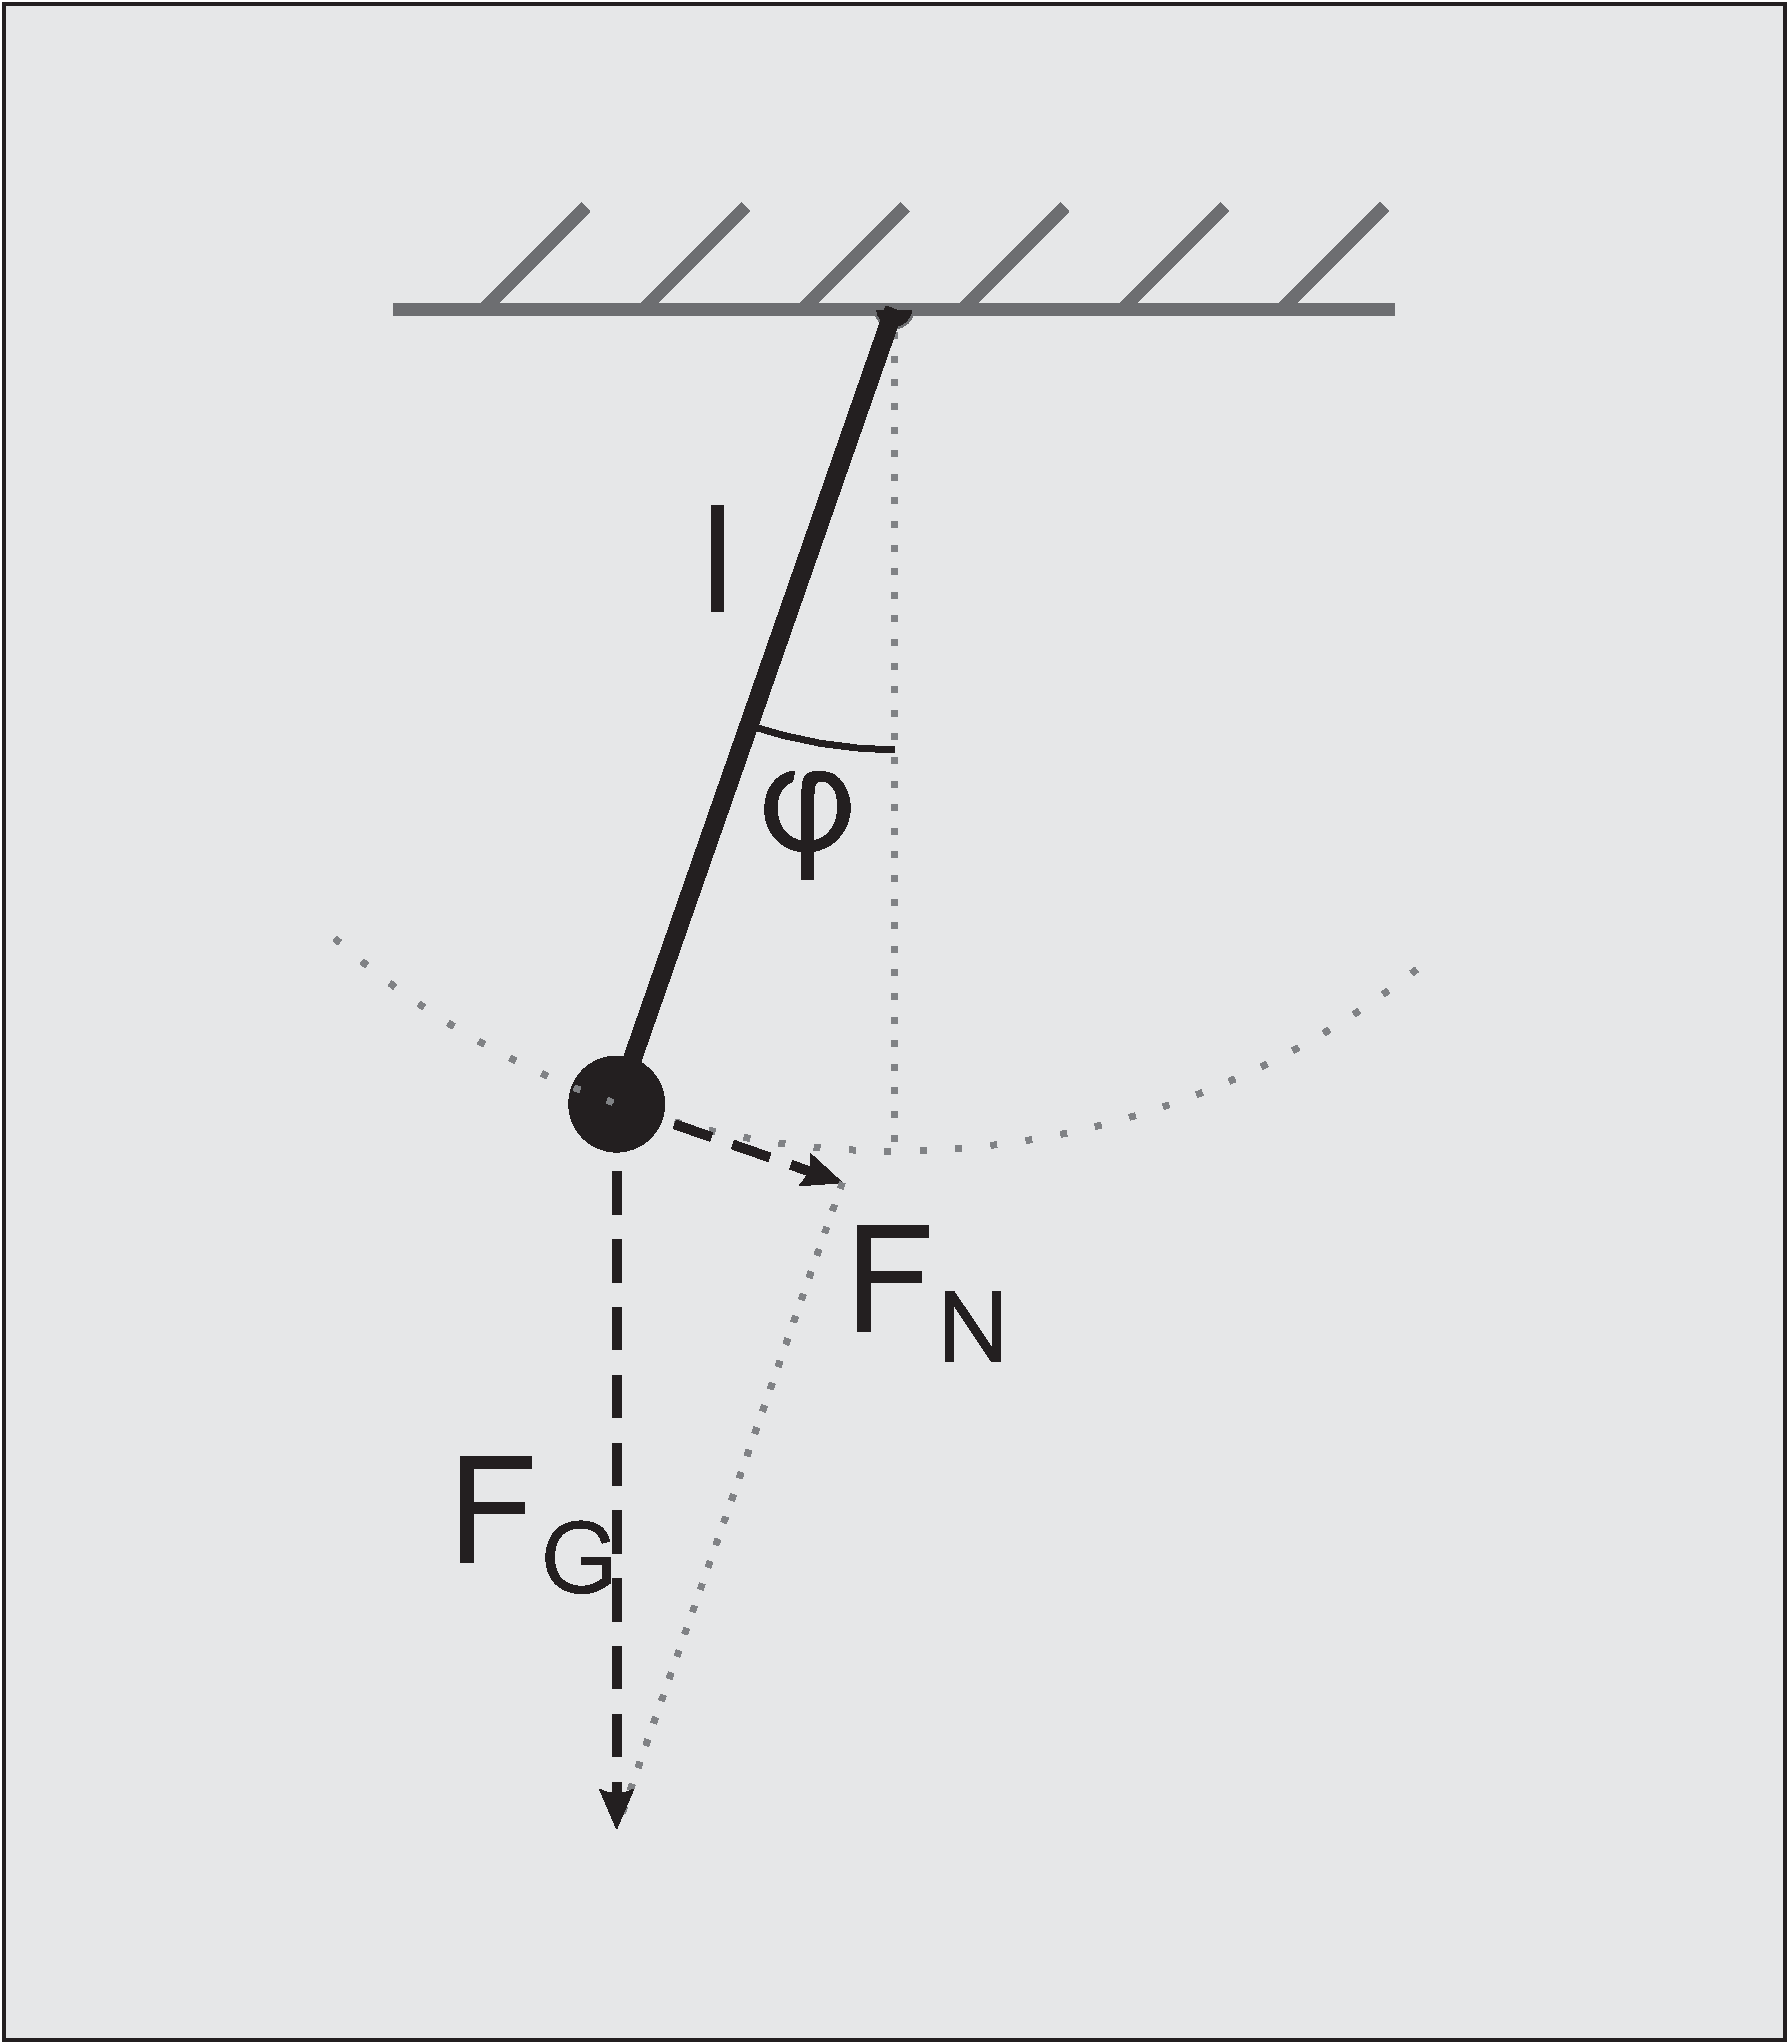
\includegraphics[draft=false,width=1.0\textwidth]{pendulum.pdf}
\end{minipage}
\hspace{2ex}
\begin{minipage}{0.5\textwidth}
 \only<1>{
 Pendulum -- Newtons law

 
 $m a = F$

 Acceleration

 $a = l \ddot{\varphi}$

 Force

 $F=F_N = - m g \sin \varphi$

 Result in an ode for the angle

 $\ddot{\varphi} = - g / l \sin \varphi $
 }

 \only<2>{

 $\ddot{\varphi} = - g / l \sin \varphi $

 Small angle $\sin \varphi \approx \phi$

 Harmonic oscillator

 $\ddot{\varphi} = - g / l \varphi$

 An analytic solution is known

 $\varphi = A \cos \omega t + B \sin \omega t$

 Amplitude $A$ and $B$ must be determined from initial conditions:

 $\varphi(t=0) = \varphi_0$, $\dot{\varphi}(t=0) = \dot{\varphi}_0$

 $B=\varphi_0$, $A=\dot{\varphi}_0 / \omega$

 }

 \only<3>{

 Full equation $\ddot{\varphi} = g / l \sin \varphi $

 has also analytic solution Jacobi elliptic function


 Lets enhance the ODE, add friction and external driving

 $\ddot{\varphi} = g / l \sin \varphi - \mu \dot{\varphi} + \varepsilon \sin \omega t $

 No analytic solution is known. We need to solve this equation numerically.
 }


 
\end{minipage}

 
\end{frame}










\frame{
  \frametitle{First example -- Lorenz system}
  \lstinputlisting{snippets/example1_a.cpp}

  \begin{itemize}
  \item The r.h.s. of the ODE is a simple function
  \item Observer
  \end{itemize}
}

\begin{frame}[fragile]{Lorenz system continued}
  % \lstinputlisting{snippets/example1_b.cpp}

  Different steppers:

  \begin{lstlisting}
runge_kutta4< state_type > stepper;
  \end{lstlisting}

  \pause
  
  \begin{lstlisting}
controlled_runge_kutta< runge_kutta_cash_karp54< state_type > > stepper;
  \end{lstlisting}

  \pause

  \begin{lstlisting}
dense_output_runge_kutta< controlled_runge_kutta<
    runge_kutta_dopri5< state_type > > > stepper;
  \end{lstlisting}

  \pause

  \begin{lstlisting}
runge_kutta_dopri5< state_type > stepper;
make_dense_output( 1.0e-6 , 1.0e-6 , stepper );    // incomplete
  \end{lstlisting}

  \pause

  All together:

  \begin{lstlisting}
int main( int argc , char **argv )
{
    state_type x = {{ 10.0 , 1.0 , 1.0 }};
    runge_kutta_dopri5< state_type > stepper;
    integrate_const( make_dense_output( 1.0e-6 , 1.0e-6 , stepper )
                     lorenz , x , 0.0 , 10.0 , 0.01 , write_lorenz );
    return 0;
}
  \end{lstlisting}



  
\end{frame}

\rem{
\frame{
  \frametitle{Side note: Templates}

  \begin{itemize}
  \item Programming paradigm: Generic programming
  \item Provide a mechanism that classes and functions work on arbitrary types
  \item Static (compile-time) polymorphism
  \item Good performance -- Compiler can optimize
  \item No virtual functions and runtime-polymorphy in odeint
  \item Concepts -- Description of requirements on the used types and classes
  \item Disadvantage: Long compilation time and memory consumption of the compiler
  \end{itemize}
}
}



\begin{frame}[fragile]{Second example -- Fermi-Pasta-Ulam lattice}
 
  \vspace{-4ex} 
 
  \begin{eqnarray}
   \dot{q}_k & = & p_k  \nonumber \\
   \dot{p}_k & = & - q_k^2 + \Delta q_k + \beta \big\{ ( q_{k+1} - q_k )^3 - ( q_k - q_{k-1} )^3 \big\} \nonumber
  \end{eqnarray}

  \centerline{\rem{Discrete Laplacian} $\Delta q_k = q_{k+1} -2 q_k + q_{k-1}$}

  \vspace{4ex}

  \pause

State type consists of coordinates $q$ and momentas $p$

  \vspace{1ex}

  \begin{lstlisting}
typedef std::vector<double> vector_type;
vector_type q( 256 ) , p( 256 );
// initialize q,p
std::pair< state_type , state_type > state = std::make_pair( q , p );
  \end{lstlisting}

  \pause

  \vspace{2ex}

  Hamiltonian system $\Longrightarrow{}$ Symplectic solvers needed

  \vspace{1ex}

  \begin{lstlisting}
symplectic_rkn_sb3a_mclachlan< vector_type > stepper;
  \end{lstlisting}


\end{frame}

\begin{frame}[fragile]{Fermi-Pasta-Ulam lattice continued}

  Trivial first component $\dot{q}_k = p_k$

  \begin{lstlisting}
struct fpu {
    double m_beta;
    fpu(double beta) : m_beta(beta) { }

    void operator()(const vector_type &q, vector_type &dpdt) const {
        // ...
    }
};
  \end{lstlisting}

  \pause

  \vspace{2ex}

  All together

  \begin{lstlisting}
struct statistics_observer {
    void operator()( const state_type &x , double t ) const { 
    // write the statistics
    }
};

int main(int argc, char **argv)
{
    vector_type q( 256 ) , p( 256 );
    // initialize q,p
    integrate_const( symplectic_rkn_sb3a_mclachlan< state_type >(), fpu(1.0),
        make_pair( q , p ), 0.0, 10.0, 0.01, statistics_observer() );
    return 0;
}
  \end{lstlisting}



\end{frame}



\section{odeint details}

\frame{\tableofcontents[currentsection]}


\frame{
  \frametitle{Structure of odeint}

  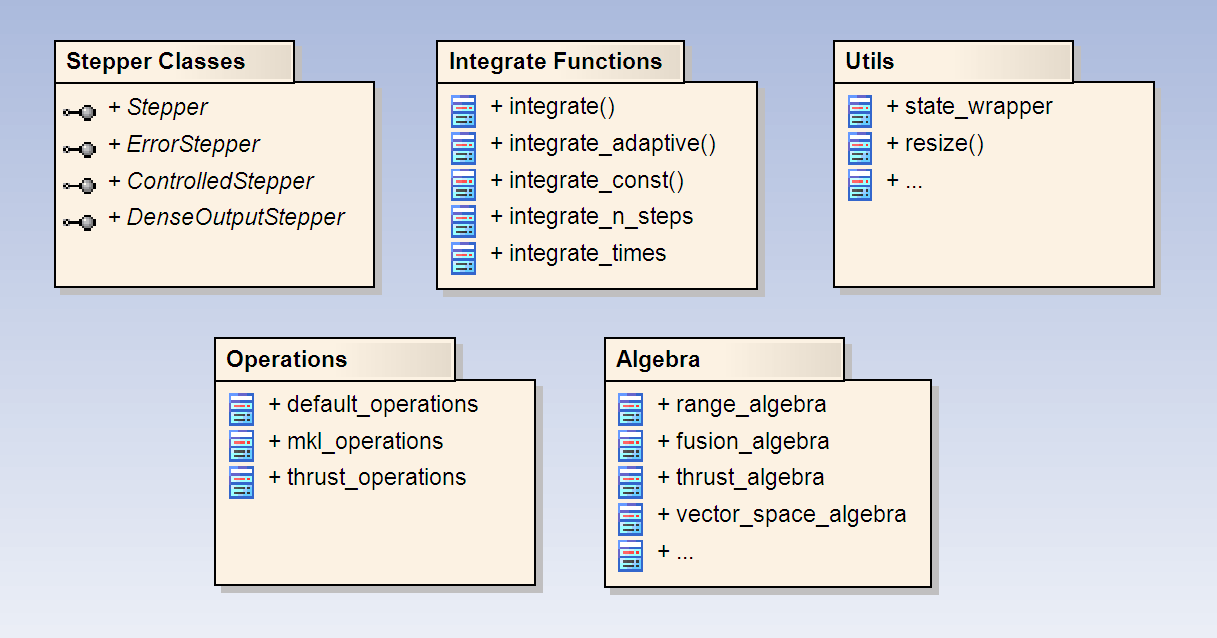
\includegraphics[draft=false,width=1.0\textwidth]{odeint_components.png}

}



\begin{frame}[fragile]
  \frametitle{Internals -- Example Euler's method}

User provides 
  \begin{displaymath}
    y_i = f_i( x(t) , t ) % \,\,\textrm{,} \quad \textrm{for all} \quad i \in (1,\dots,N)
  \end{displaymath}

odeint provides
  \begin{displaymath}
    x_i (t + \Delta t ) = x_i( t )  + \Delta t \cdot y_i
  \end{displaymath}

(In general vector operations like $\,\, z_i = a_1 x_{1,i} + a_2 x_{2,i} + \dots $)



\vspace{4ex}

Instantiation

\vspace{1ex}

\begin{lstlisting}[basicstyle=\small\ttfamily,escapechar=!]
euler<state_type, value_type, deriv_type, time_type, algebra, operations > stepper;
\end{lstlisting}

\vspace{1ex}

{\bf All elements for container independence and portability are already included in this line!}

\end{frame}

\begin{frame}[fragile]
  \frametitle{Internals -- Example Euler's method}

  \begin{displaymath}
    y_i = f_i( x(t) )
  \end{displaymath}
  \begin{displaymath}
    x_i (t + \Delta t ) = x_i( t )  + \Delta t \cdot y_i
  \end{displaymath}

\vspace{2ex}

\begin{lstlisting}[basicstyle=\small\ttfamily]
euler<state_type, value_type, deriv_type, time_type, algebra, operations > stepper;
\end{lstlisting}

\vspace{2ex}

\begin{overlayarea}{\textwidth}{10cm}
 \rem{\only<1>{General goal: Separation 
  \begin{itemize}
   \item of how an vector is iterated
   \item of how the basic computations are performed
  \end{itemize}
from the stepper
 }}
\rem{ \only<1>{Examples:

  {\tt \scriptsize euler<vector<double>, double, vector<double>, double ,
range\_algebra, default\_operations>;}

\vspace{1ex}

  {\tt \scriptsize euler<vector<complex<double> >, double, vector<complex<double> >, double ,
range\_algebra, default\_operations>;}  

  {\tt \scriptsize euler<thurst::device\_vector<double>, double, thrust::device\_vector<double>, double ,
thrust\_algebra, thrust\_algebra>;} 
}}
 \only<1>{
 Data types
 \begin{itemize}
  \item {\tt state\_type} -- the type of $x$
  \item {\tt value\_type} -- the basic numeric type, e.g. {\tt double}
  \item {\tt deriv\_type} -- the type of $y$
  \item {\tt time\_type} -- the type of $t$, $\Delta t$
 \end{itemize}}
 \only<2>{
 Algebra policies, perform the iteration

 \vspace{2ex}

 Algebra must be a class with public methods
 \begin{itemize}
 \item {\tt for\_each1(x,op)} -- Performs $op(x_i)$ for all $i$
 \item {\tt for\_each2(x1,x2,op)} -- Performs $op(x1_i,x2_i)$ for all $i$
 \item ...
 \end{itemize}}
 \only<3>{
 Operations do the basic computation

 \vspace{2ex}

 Operations must be a class with the public classes (functors)
 \begin{itemize}
 \item {\tt scale\_sum1} -- Calculates $x = a1 \cdot y1 $
 \item {\tt scale\_sum2} -- Calculates $x = a1 \cdot y1 + a2 \cdot y2$
 \item ...
 \end{itemize}}
 \only<4>{
 All together

\vspace{2ex}
   {\tt \scriptsize m\_algebra.for\_each3(xnew ,xold, y ,\\
\hspace{4ex}operations\_type::scale\_sum2<value\_type,time\_type>(1.0,dt));}
}
\end{overlayarea}


\end{frame}




\frame{
  \frametitle{Stepper concepts}

  \begin{block}{Concepts}
    ``... In generic programming, a concept is a description of supported
    operations on a type...''
  \end{block}

  \pause
  \vspace{4ex}
  odeint provides
  \begin{itemize}
   \item Stepper concept \\ \lstinline[basicstyle=\small\ttfamily]+stepper.do_step(sys,x,t,dt);+
   \item ErrorStepper concept \\ \lstinline[basicstyle=\small\ttfamily]+stepper.do_step(sys,x,t,dt,xerr);+
   \item ControlledStepper concept \\ \lstinline[basicstyle=\small\ttfamily]+stepper.try_step(sys,x,t,dt);+
   \item DenseOutputStepper concept \\ \lstinline[basicstyle=\small\ttfamily]+stepper.do_step(sys);+ \\ \lstinline[basicstyle=\small\ttfamily]+stepper.calc_state(t,x);+
  \end{itemize}

}

\rem{
\frame{
  \begin{block}{Concepts}
    ``... In generic programming, a concept is a description of supported
    operations on a type...''
  \end{block}
  \begin{columns}[t]
    \begin{column}{0.32\textwidth}
      \begin{block}{Stepper}
        {\footnotesize
          provides method:
          {do\_step(sys,x,t,dt)}

        \vspace{1ex}

        Performs one time step with constant step size

        \vspace{1ex}

        Example:

        stepper\_rk4<vector>~rk;

        ...

        rk.do\_step(lor,x,t,dt);
        }
      \end{block}
    \end{column}
    \begin{column}{0.32\textwidth}
      \begin{block}{Error stepper}
        {\footnotesize
          provides method:
          {do\_step(sys,x,t,dt,xerr)}

        \vspace{1ex}

        Performs one time step with constant step size and error estimation

        \vspace{1ex}

        Example:

        stepper\_rk5\_ck<..>~rk;

        ...

        rk.do\_step(lor,x,t,dt,xerr);}
      \end{block}
    \end{column}
    \begin{column}{0.32\textwidth}
      \begin{block}{Controlled stepper}
        {\footnotesize
          provides method:
          {try\_step(sys,x,t,dt)}

        \vspace{1ex}

        Tries to performs one time step within a given accuracy. Suggests new
        step size.

        \vspace{1ex}

        Example:

        controlled\_stepper\_bs;
        }
      \end{block}
    \end{column}
  \end{columns}

  Dense output concept
}
}

\frame{
  \frametitle{Supported methods}
    {\scriptsize
    \begin{tabular}{lll}
      {\bf Method} & {\bf Class name} & {\bf Concept} \\
      Euler & {\tt euler} & SD \\
      Runge-Kutta 4 & {\tt runge\_kutta4} & S \\
      Runge-Kutta Cash-Karp & {\tt runge\_kutta\_cash\_karp54} & SE \\
      Runge-Kutta Fehlberg & {\tt runge\_kutta\_runge\_fehlberg78} & SE \\
      Runge-Kutta Dormand-Prince & {\tt runge\_kutta\_dopri5} & SED \\
      & & \\
      Runge-Kutta controller & {\tt controlled\_runge\_kutta} & C \\
      Runge-Kutta dense output & {\tt dense\_output\_runge\_kutta} & D \\
      & & \\
      Symplectic Euler & {\tt symplectic\_euler} & S \\
      Symplectic RKN & {\tt symplectic\_rkn\_sb3a\_mclachlan} & S \\
      & & \\
      Rosenbrock 4 & {\tt rosenbrock4} & ECD \\
      Implicit Euler & {\tt implicit\_euler} & S \\
      & & \\
      Adams-Bashforth-Moulton & {\tt adams\_bashforth\_moulton} & S \\
      Bulirsch-Stoer & {\tt bulirsch\_stoer} & CD 
    \end{tabular}

    \vspace{4ex}

    S -- fulfills stepper concept

    E -- fulfills error stepper concept

    C -- fulfills controlled stepper concept

    D -- fulfills dense output stepper concept

  }
}






\frame{
  \frametitle{Integrate functions}

  \begin{itemize}
   \item {\tt integrate\_const}
   \item {\tt integrate\_adaptive}
   \item {\tt integrate\_times}
   \item {\tt integrate\_n\_steps}
  \end{itemize}

  Perform many steps, use all features of the underlying method

  \vspace{2ex}

  \pause

  An additional observer can be called

  \vspace{2ex}

  {\tt integrate\_const(stepper, sys, x, t\_start, t\_end, dt, obs);}

}





\frame{
  \frametitle{More internals}
    \begin{itemize}
      \item Header-only, no linking $\rightarrow$ powerful compiler optimization
      \item Memory allocation is managed internally
      \item No virtual inheritance, no virtual functions are called
      \item Different container types are supported, for example
        \begin{itemize}
          \item STL containers ({\tt vector}, {\tt list}, {\tt map}, {\tt tr1::array})
          \item MTL4 matrix types, blitz++ arrays, Boost.Ublas matrix types
          \item {\tt thrust::device\_vector}
          \item Fancy types, like Boost.Units
          \item ANY type you like
        \end{itemize}
      \item Explicit Runge-Kutta-steppers are implemented with a new template-metaprogramming method
      \item Different operations and algebras are supported
        \begin{itemize}
          \item MKL
          \item Thrust
          \item gsl
        \end{itemize}
    \end{itemize}
}


\frame{
  \frametitle{ODEs on GPUs}

  Graphical processing units (GPUs) are able to perform up to $10^6$ operations at once in parallel
 
  \vspace{2ex}

  Frameworks
  \begin{itemize}
   \item CUDA from NVIDIA
   \item OpenCL
   \item Thrust a STL-like library for CUDA and OpenMP
  \end{itemize}

  \vspace{2ex}

  Applications:
  \begin{itemize}
   \item Parameter studies
   \item Large systems, like ensembles or one- or two dimensional lattices
   \item Discretizations of PDEs
  \end{itemize}

  \vspace{2ex}

  {\bf odeint supports CUDA, through Thrust}
}

\frame{
  \frametitle{Example: Parameter study of the Lorenz system}

  \lstinputlisting{snippets/example3_thrust.cpp}
}




\section{Outlook and conclusion}

\frame{
  \frametitle{Conclusion}

  \begin{itemize}
    \item odeint provides a fast, flexible and easy-to-use C++ library for
      numerical integration of ODEs.
    \item Its container independence is a large advantage over existing
      libraries.
    \item Portable
    \item Generic programming is the main programming technique.
  \end{itemize}

}



\frame{
  \frametitle{Outlook}
  \begin{itemize}
    \item Submission to the boost libraries
    \item Dynamical system classes for easy implementation of interacting dynamical systems
    \item More methods: implicit methods and multistep methods.
    \item Implementation of the Taylor series method
  \end{itemize}

  \vspace{4ex}

  \lstinputlisting{snippets/example4_lorenz_taylor.cpp}
}



\frame{
  \frametitle{Resources}

Download and documentation

{\tt odeint.com}

\vspace{2ex}

An article about the used techniques exists at

{\tt \small http://www.codeproject.com/KB/recipes/odeint-v2.aspx}

\vspace{2ex}

Development

{\tt https://github.com/headmyshoulder/odeint-v2}

\vspace{4ex}

\begin{block}{Contributions and feedback}
 are highly welcome
\end{block}





}


\end{document}
